% Tipo de documento
\documentclass[12pt,twocolumn,a4paper]{report}
% UTF-8 and friends
\usepackage[utf8]{inputenc}
\usepackage[spanish]{babel}
\usepackage{titlesec}
\usepackage{titletoc}
\usepackage{hyperref}
\usepackage{lipsum}
\usepackage{multicol}
\usepackage{graphicx}
\usepackage{float}
\usepackage{amsmath}
\usepackage{vmargin}
\usepackage{longtable}
\newtheorem{ejemplo}{Ejemplo}
\newtheorem{mydef}{Definition}
\usepackage{tcolorbox}
\tcbuselibrary{theorems}
\usepackage[colorinlistoftodos,textwidth=2cm,shadow]{todonotes}
\setpapersize{A4}
\setmargins{2.5cm}       % margen izquierdo
{1.5cm}                        % margen superior
{16.5cm}                      % anchura del texto
{23.42cm}                    % altura del texto
{10pt}                           % altura de los encabezados
{1cm}                           % espacio entre el texto y los encabezados
{0pt}                             % altura del pie de página
{2cm}                           % espacio entre el texto y el pie de página
% Para los capitulos
%\titleformat{\chapter}[display]
%{\bfseries\huge\bfseries\filcenter}{\thechapter}{25pt}{\Large}
% [%
%  \startcontents
%  \printcontents{}{1}{\setcounter{tocdepth}{3}}%
%  ]
\title{Apuntes de Estadística}
\author{Joaquín Escalona}
\date{}

\begin{document}
\maketitle

\newpage
\tableofcontents

%----------------------------------------------------
\onecolumn

\chapter*{Introducción}
\addcontentsline{toc}{chapter}{Introducción}
La estadística es una ciencia que nos facilita numerosas herramientas para abordar de manera óptica todas las etapas necesarias, hasta una interpretación final buena de los datos, que a su vez guardan relación con el interés de nuestro estudio.

Las etapas a considerar se basan básicamente en reunir, resumir y clasificar los datos para luego ser analizados e interpretados.

En resumen es:

Obtenemos datos, analizamos los datos y finalmente presentamos conclusión referente a la información de interés.

\twocolumn

\chapter*{Tipos de datos}
\addcontentsline{toc}{chapter}{Tipos de datos}
En estricto rigor, un dato es un valor (o resultado) de una variable. Por ejemplo, si preguntamos a una persona ?`Cuántos hermanos tiene? y esta contesta $2$, entonces la variable es 'N$^{\circ}$ de hermanos' y el dato obtenido es 2. 

Las variables pueden ser clasificadas en dos grandes grupos:
\section*{Variables cualitativas}
\addcontentsline{toc}{section}{Variables cualitativas}
Estas denotan una cualidad (Ej: Tamaño de un arbol: Alto, mediano, bajo; Color de un vehículo: Verde,azul,rojo; etc...)

Las variables cualitativas a su vez pueden ser clasificadas en
dos sub-grupos:
\begin{itemize}
\setlength\itemsep{0.001cm}
\item{\textbf{Nominales:}Sus resultados son representados por números o letras y el orden de clasificacion \textbf{NO} importa (Ej: La variable 'Color de un vehículo' puede tener resultados V:Verde, A:Amarillo, R:Rojo).}
\item{\textbf{Ordinales}Sus resultados son representados por números o letras y el orden de clasificación \textbf{SI} importa (Ej: La variable 'Tamaño de un árbol' puede tener por resultado 1:Alto, 2:Mediano, 3:Bajo).}
\end{itemize}

\section*{Variables cuntitativas}
\addcontentsline{toc}{section}{Variables cuntitativas}
Estas denotan una cantidad (Ej: El N$^{\circ}$ de hermanos: 0,1,2...; Peso; Estatura;etc...)
Las variables cuantitativas a su vez pueden ser clasificadas en dos sub-grupos:
\begin{itemize}
\setlength\itemsep{0.001cm}
\item{\textbf{Discretas:}Sus resultados toman valores enteros pues surgen de un procedimiento de conteo.}
\item{\textbf{Continuas:}Sus resultados toman valores dentro de un intervalo y surgen de un procedimiento de medición}
\end{itemize}

A modo de resumen: 
\begin{figure}[H]
\centering
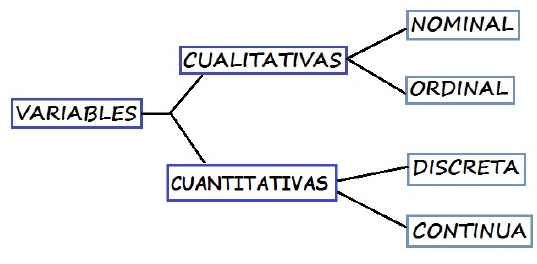
\includegraphics[scale=0.5]{graficos/1.png}
\end{figure}

\onecolumn
\chapter*{Algunas definiciones}
\addcontentsline{toc}{chapter}{Algunas definiciones}
\section*{Población}
\addcontentsline{toc}{section}{Población}
Conjunto de todos los individuos u objetos que tienen al menos una característica en común. (Ej: Peso de los niños en Chile
\section*{Parámetro}
\addcontentsline{toc}{section}{Parámetro}
Medida resumen que describe alguna característica del total de la población.

\section*{Muestra}
\addcontentsline{toc}{section}{Muestra}
Subconjunto de la población y es obtenida por medio de un muestreo. 

\section*{Estadístico o Estadigrafo}
\addcontentsline{toc}{section}{Estadístico o Estadigrafo}
Una medida que describe alguna característica de la muestra (Ej: Estatura media de la muestra).

\twocolumn

\chapter*{Representación de variables}
\addcontentsline{toc}{chapter}{Representación de variables}
Surge una pregunta acerca de cómo podemos resumir la información que tenemos en un problema particular con varios datos.

Las opciones son

\section*{Tablas de frecuencias}
\addcontentsline{toc}{section}{Tablas de frecuencias}
Supongamos que contamos con $n$ observaciones de la variable aleatoria X. Diremos que $n$ es el \textbf{tamaño de la muestra.}

La representación tabular o bien \textbf{Tabla de frencuencias} de las variables no es mas que un resumen en forma de tabla de la información de los datos obtenidos. 

Para construir una tabla de frencuencias debemos tener en claro las siguientes definiciones:
\begin{itemize}
\setlength\itemsep{0.001cm}
\item{\textbf{Frencuencia absoluta($n_i$):} Es el número de veces que se repite un valor de una variable estadística que llamaremos $x_i$.Notemos que la suma de éstas frencuencias será igual al tamaño muestral $n$}
\item{\textbf{Frecuencia absoluta acumulada ($N_i$): }Es el número de veces que se repite un valor menor o igual a $x_i$ de una variable estadística.}
\item{\textbf{Frecuencia relativa ($f_i$):} Es la proporción en que está representado el valor $x_i$ sobre el total de $n$ muestras. Es decir, $$f_i = \dfrac{n_i}{n}$$}
\item{\textbf{Frecuencia relativa acumulada ($F_i$):} Es la proporción en que está representado un valor menor o igual a $x_i$ sobre el total de $n$ muestras. Es decir, $$F_i = \dfrac{N_i}{n}$$}
\item{\textbf{Frecuencia relativa porcentual o Porcentaje (\%$f_i$)}:} Es el porcentaje en que está representado el valor $x_i$ sobre el total de $n$ muestras. Es decir, $$\% f_i = 100 \times f_i $$
\end{itemize}

\todo[inline,backgroundcolor = green!10]{Para \textbf{variables cualitativas} no tiene sentido las frecuencias acumuladas}

\begin{ejemplo}
\label{ej1}
Los siguientes datos son los computadores fabricados por la empresa Dell: 
\begin{figure}[H]
\centering
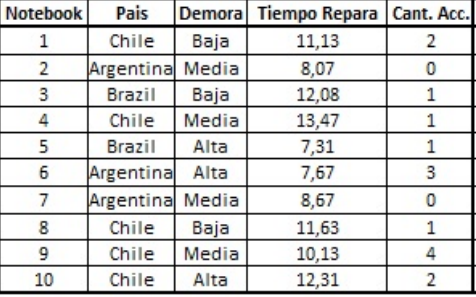
\includegraphics[scale=0.5]{graficos/2.png}
\end{figure}

\begin{figure}[H]
\centering
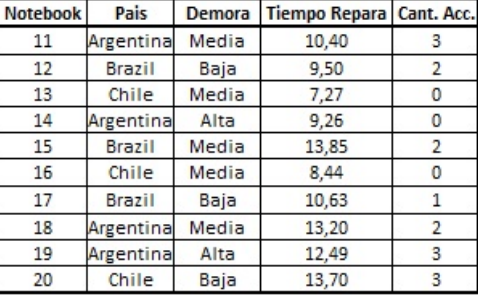
\includegraphics[scale=0.5]{graficos/3.png}
\end{figure}
\end{ejemplo}
\newpage
Para variable cualitativa nominal
\begin{table}[H]
\begin{tabular}{|l|l|l|l|}
\hline
País      & $n_i$ & $f_i$          & $f_i\%$                  \\ \hline
Chile     & 8     & $\frac{8}{20}$ & $100\times \frac{8}{20}$ \\ \hline
Brazil    & 5     & $\frac{5}{20}$ & $100\times \frac{5}{20}$ \\ \hline
Argentina & 7     & $\frac{7}{20}$ & $100\times \frac{7}{20}$ \\ \hline
\end{tabular}
\end{table}
Para variable cualitativa ordinal 
\begin{table}[H]
\begin{tabular}{|l|l|l|l|}
\hline
Cant. Acc & $n_i$ & $f_i$          & $f_i\%$ \\ \hline
0         & 5     & $\frac{5}{20}$ & $25 \%$ \\ \hline
1         & 5     & $\frac{5}{20}$ & $25 \%$ \\ \hline
2         & 5     & $\frac{5}{20}$ & $25 \%$ \\ \hline
3         & 4     & $\frac{4}{20}$ & $20 \%$ \\ \hline
3         & 1     & $\frac{1}{20}$ & $5\%$   \\ \hline
\end{tabular}
\end{table}

\todo[inline,backgroundcolor = green!10]{En el caso de variables cuantitativas continuas, dado que hay muchos valores posibles para la variable, agrupemos valores en intervalos que llamaremos \textbf{intervalos de clase}}

\subsection*{Intervalos de clase}
\addcontentsline{toc}{subsection}{Intervalos de clase}
Para la construcción de los intervalos de clase, será necesario considerar las siguientes definiciones:
\begin{itemize}
\setlength\itemsep{0.001cm}
\item{\textbf{Clase:} Es el intervalo en que cae cada dato}
\item{\textbf{Marca de clase ($x_i$):} Corresponde al punto medio de cada clase (Es el representante de cada clase)}
\item{\textbf{Rango (R):} Es la distancia que existe entre valor mínimo y valor máximo de los datos de la muestra. Es decir, $R = X_{(n)}-X_{(1)} = x_{max}-x_{min}$}
\item{\textbf{Amplitud (A):} Es el tamaño de cada intervalo, se define como $A = \dfrac{R}{k}$} 
\end{itemize}

Ahora bien, es válido preguntarse, `Si dispongo de una muestra de tamaño $n$, ?`Cuántas clases (intervalos debemos considerar? Para ello, debemos emplear la \textbf{Regla de Sturgess}, que se define como $$ k = 1 + 3.322 \enspace log(n) $$

\begin{ejemplo}
con los datos del ejemplo anterior \ref{ej1} construiremos la tabla de frencuencia para las variables continuas  
\end{ejemplo}
\begin{figure}[H]
\centering
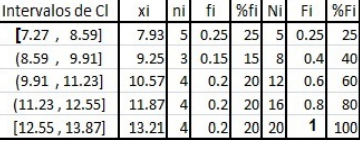
\includegraphics[scale=0.7]{graficos/4.png}
\end{figure}

\section*{Otros graficos}
\addcontentsline{toc}{section}{Otros graficos}
\todo[inline,backgroundcolor = green!10]{Para variables cualitativas se usan gráficos \textbf{de torta / barra} y para las cuantitativas se usa el \textbf{histograma / boxplot }}
\begin{figure}[H]
\centering
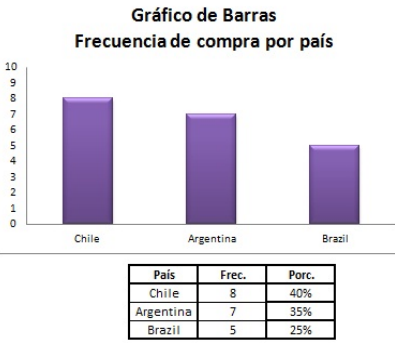
\includegraphics[scale=0.5]{graficos/5.png}
\end{figure}
\begin{figure}[H]
\centering
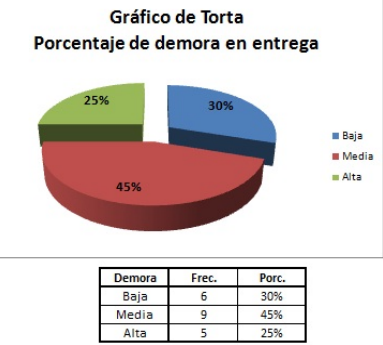
\includegraphics[scale=0.5]{graficos/6.png}
\end{figure}

\chapter*{Medidas de tendencia central}
\addcontentsline{toc}{chapter}{Medidas de tendencia central}

\section*{Promedio}
\addcontentsline{toc}{section}{Promedio}
La media o promedio de una muestra $x_1,... ,x_n$ se define como: 
\begin{equation*}
\bar{X}= \left\{ \begin{array}{lc}
             \frac{1}{n}\sum_{i=1}^{n}x_i  & \text{Datos no tabulados} \\
             \\ \frac{1}{n}\sum_{j=1}^{k}n_j x_j  & \text{Datos tabulados} 
             \end{array}
   \right.
\end{equation*}
Note que para el caso de datos tabulados (agrupados) SIN intervalos, $x_j$ representa una clase (valor) en particular y para el caso de datos tabulados (agrupados) CON intervalos, $x_j$ representa la marca de clase. 

\section*{Mediana}
\addcontentsline{toc}{section}{Mediana}
La mediana de un conjunto de observaciones se define como aquel valor que no es superado ni supera a más de la mitad de las observaciones ordenadas de forma creciente (es el dato que está en el centro de los datos de la muestra). La mediana no es afectada por valores extremos como sucede en el caso de la media y se calcula de manera diferente si las observaciones se encuentran agrupadas o no.

En el caso que las observaciones NO estén agrupadas, primero debemos ordenarlas de menor a mayor. 

Luego la mediana se obtiene como 

\begin{equation*}
Me= \left\{ \begin{array}{lc}
             X_{\left(\frac{n+1}{2}\right)} & \text{n impar} \\
             \\ \frac{X_{\left(\frac{n}{2}\right)}+X_{\left(\frac{n}{2}+1\right)}}{2} & \text{n par}
             \end{array}
   \right.
\end{equation*}

En el caso de que los datos estén agrupados en una tabla de frencuencia, habrá que hacer distinción entre datos tabulados CON o SIN intervalos.

Para el caso de datos tabulados SIN intervalos la mediana la calculamos de la siguiente manera:
\begin{equation*}
Me= \left\{ \begin{array}{lcc}
             x_j & si & N_{j-1} < \frac{n}{2} < N_j \\
             \\ \frac{x_{j-1}+x_j}{2} & si & \frac{n}{2} = N_{j-1}
             \end{array}
   \right.
\end{equation*}
donde $N_{j-1}$ es la frecuencia acumulada del intervalo anterior al que contiene la mediana. 

Para el caso de datos tabulados CON intervalos la mediana la calculamos de la siguiente manera: 
Buscamos el intervalo que contiene al dato que ocupa la posición $\frac{n}{2}$,esto de forma similar al procedimiento descrito para datos tabulados sin intervalos. Luego calculamos la mediana como: 

\begin{equation*}
    Me = L_{inf,j} + \frac{\dfrac{n}{2}- N_{j-1}}{{n_j}}A_j 
\end{equation*}

Donde: 
\begin{itemize}
\setlength\itemsep{0.001cm}
\item{$L_{inf,j}$: Límite inferior del intervalo que contiene la mediana}
\item{$N_{j-1}$: frecuencia acumulada del intervalo anterior al que contiene la mediana.}
\item{$n_j$: frecuencia absoluta del intervalo que contiene la mediana.}
\item{$A_j$: amplitud del intervalo que contiene la mediana.}
\end{itemize}

\section*{Moda}
\addcontentsline{toc}{section}{Moda}
La moda de un conjunto de datos es el valor que más se repite. Notemos que ésta no necesariamente es única y se obtiene de forma natural tanto para el caso en que se tienen datos cualitativos como cuantitivos no tabulados o tabulados SIN intervalos. 

En el caso que se tengan datos tabulados CON intervalos, debemos encontrar una aproximación de la moda, la cual calculamos de la siguiente manera: 

Buscamos el (los) intervalos que contienen a la moda al que llamaremos \textbf{clase modal}. Luego calculamos la moda como: 

\begin{equation*}
Mo = L_{inf,j} + \frac{n_j - n_{j-1}}{(n_j - n_{j-1})+(n_j - n_{j+1})} A_j 
\end{equation*}
\begin{itemize}
\setlength\itemsep{0.001cm}
\item{$L_{inf,j}$: límite inferior de la clase modal.}
\item{$n_j$: frecuencia absoluta de la clase modal.}
\item{$A_j$: amplitud de la clase modal. }
\end{itemize}

\section*{Percentiles}
\addcontentsline{toc}{section}{Percentiles}
Se divide a la muestra \textbf{ordenada} en 100 partes iguales y es tal que el i-ésimo percentil ($P_i$ es un valor donde al menos un $i\%$ de los datos están bajo su valor y el restante (100-i)\% por encima de él. 

Los percentiles se calculan de manera diferente si las observaciones se encuentran agrupadas o no.

\subsection*{Datos no agrupados}
\addcontentsline{toc}{subsection}{Datos no agrupados}
En el caso de que las observaciones \textbf{NO} estén agrupadas, primero debemos ordenarlas de menor a mayor. 

Luego, el percentil i-ésimo se obtiene como
\begin{equation*}
P_i= \left\{ \begin{array}{lcc}
             x_{\left[\frac{i\cdot n}{100}\right]} & si & \frac{i\cdot n}{100} \text{es fraccion} \\
             \\ (x_{\frac{i\cdot n}{100}}+x_{\frac{i\cdot n}{100}+1})/2 & si & \frac{i\cdot n}{100} \text{es entero}
             \end{array}
   \right.
\end{equation*}

Donde [q] es el entero próximo mayor a la fracción q. 

\subsection*{Datos agrupados}
\addcontentsline{toc}{subsection}{Datos agrupados}
En el caso de que los datos estén agrupados en una tabla de frencuencias, habrá que hacer distinción entre datos tabulados CON o SIN intervalos. 

Para el caso de datos tabulados \textbf{SIN} intervalos, el percentil $P_i$ será calculado de la siguiente manera:
\begin{equation*}
P_i= \left\{ \begin{array}{lcc}
             x_j & si & N_{j-1} < \frac{i \cdot n}{100} < N_j \\
             \\ \frac{x_j + x_{j+1}}{2} & si & \frac{i\cdot n}{100} = N_j
             \end{array}
   \right.
\end{equation*}
donde $N_{j-1}:$ frecuencia acumulada del intervalo anterior al que contiene la mediana. 

Para el caso de datos tabulados \textbf{CON} intervalos el percentil $P_i$ será calculado de la siguiente manera. 

Buscamos el intervalo que contiene al dato que ocupa la posición $\dfrac{i \ cdot n}{100}$

\begin{equation*}
P_i = L_{inf,j} + \frac{\dfrac{i \cdot n}{100} - N_{j-1}}{n_j} A_j
\end{equation*}
donde: 
\begin{itemize}
\setlength\itemsep{0.001cm}
\item{$L_{inf,j}$: límite inferior que contiene el $P_i$.}
\item{$N_{j-1}$: frecuencia acumulada del intervalo anterior al que contiene el $P_i$.}
\item{$n_j$: frecuencia absoluta del intervalo que contiene el $P_i$}
\item{$A_j$: amplitud del intervalo que contiene el $P_i$. }
\end{itemize}

\subsection*{BoxPlot}
\addcontentsline{toc}{subsection}{BoxPlot}
En este gráfico es posible observar características de los datos como simetría y posibles observaciones atípicas. 

Para construir un boxplot es necesario delimitar los límites admisibles tal que fuera de ellos consideraremos que los datos son atípicos (datos outliers). Estos se calculan como: 

Límite inferior (L.I) = $Q_1 - f(Q_3 - Q_1)$ \\
Límite Superior (L.S) = $Q_3 + f(Q_3 - Q_1$ 

Donde, en general se considera $f = 0.75 $ o 1.5 

El boxplot entonces tendrá la siguiente forma: 
\begin{figure}[H]
\centering
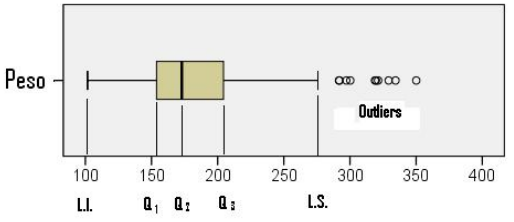
\includegraphics[scale=0.5]{graficos/7.png}
\end{figure}


\chapter*{Medidas de dispersión}
\addcontentsline{toc}{chapter}{Medidas de dispersión}

\section*{Rango Intercuartil y Varianza}
\addcontentsline{toc}{section}{Rango Intercuartil y Varianza}
El rango intercuartil (R.I) es la longitud del intervalo donde están concentrados el 50\% central de los datos, es decir, $$R.I = Q_3 - Q_1$$

La varianza de una muestra, denotada por $s^2$ se define como la media del cuadrado de las desviaciones de los datos con respecto al promedio de éstos. En términos numéricos, se obtiene de la siguiente manera: 
\begin{equation*}
s^2= \left\{ \begin{array}{lc}
             \frac{1}{n-1}\sum_{i = 1}^{n} (x_i - \bar{x})^2 & \text{Datos NO agrupados} \\
             \\ \frac{1}{n-1}\sum_{j = 1}^{k} (x_j - \bar{x})^2  & \text{Datos agrupados}
             \end{array}
   \right.
\end{equation*}

\section*{Desviación estándar}
\addcontentsline{toc}{section}{Desviación estándar}
Un posible inconveniente de la varianza es que las unidades de medida quedan elevadas al cuadrado, por lo que esta interpretación de dispersión no es muy natural. 

La desviación estándar de una muestra se denota por $s$ y se obtiene como la raíz cuadrada de la varianza $s^2$: $$s = \sqrt{s^2} $$

\section*{Coeficiente de variación}
\addcontentsline{toc}{section}{Coeficiente de variación}
Es una medida de dispersión que es adimensional pues está definido por: $$ CV = \frac{s}{\bar{x}} $$

Dado que es adimensional, permite comparar la dispersión de dos conjuntos de datos que no tengan la misma unidad de medida. 




\chapter*{Estadística}
\addcontentsline{toc}{chapter}{Estadística}

Si usted compra un boleto de Kino o bien invierte en acciones de alguna empresa, no sabe a ciencia cierta si es que va a obtener ganancias o pérdidas. 

Lo que intentamos hacer con el cálculo de probabilidades es cuantificar la incertidumbre asociada a ganar el Kino o, en el otro caso, la probabilidad de ganar una cierta cantidad de dinero al comprar la acción. 

Intentamos indicar cuán factible es que ocurra algún resultado en particular como consecuencia de un \textbf{experimento aleatorio.}

\section*{Definiciones}
\addcontentsline{toc}{section}{Definiciones}

\subsection*{Experimento aleatorio}
\addcontentsline{toc}{subsection}{Experimento aleatorio}
Un experimento aleatorio es cualquier experimento cuyo resultado es incierto, no se conoce con seguridad. Denotaremos a cualquier experimento aleatorio como $\epsilon$

Ejemplos de experimentos aleatorios:
\begin{itemize}
\setlength\itemsep{0.001cm}
\item{Lanzamiento de una moneda}
\item{lanzamiento de un dado}
\item{género de un alumno(a) seleccionado en el curso}
\end{itemize}

\subsection*{Espacio muestral}
\addcontentsline{toc}{subsection}{Espacio muestral}
Decimos que el conjunto $S_\epsilon$ es el espacio muestral del experimento $\epsilon$ si $S$ contiene a \textbf{TODOS} los posibles resultados del experimento $\epsilon$

Algunos ejemplos de espacios muestrales son los siguientes:
\begin{figure}[H]
\centering
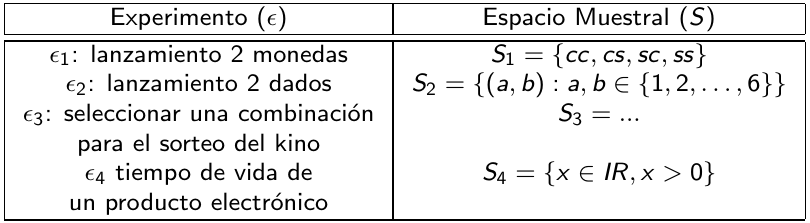
\includegraphics[scale=0.3]{graficos/8.png}
\end{figure}

\subsection*{Evento}
\addcontentsline{toc}{subsection}{Evento}
Un evento es cualquier colección de posibles resultados de un experimento. 

Consideremos el experimento del lanzamiento de dos dados. El espacio muestral esta dado por 
$$ 
S\{(a,b): a,b \in \{1,2,...,6\}\}
$$
Sea el evento $A =$ la suma de las caras superiores sea a lo más 4. Por lo tanto 
$$
A = \{(1,1); (1,2); (1,3); (2,1); (3,1); (2,2)\}
$$
Notemos que $A$ es un subconjunto de $S$.

Decimos que el evento $A$ ocurre si el resultado del experimento está en el conjunto $A$. 

Sea $A$ un evento cualquiera asociado al experimento $\epsilon$. Por definición, $A$ es \textbf{siempre un subconjunto} del espacio muestral $S_\epsilon$, es decir
$$
A \subset S \Longleftrightarrow x \in A \Rightarrow x \in S
$$

\subsection*{Evento unión}
\addcontentsline{toc}{subsection}{Evento unión}
Sean $A$ y $B$ dos eventos definidos sobre el espacio muestral $S$. El evento definido por la unión de $A$ y $B$, denotado por $A \cup B$, contiene al conjunto de elementos que están o bien en $A$, o bien en $B$, o bien en ambos eventos. 
$$
A \cup B = \{x: x \in A \vee x \in B \}
$$

\subsection*{Evento intersección}
\addcontentsline{toc}{subsection}{Evento intersección}
Sean $A$ y $B$ dos eventos definidos sobre el espacio muestral $S$. El evento definido por la intersección de $A$ y $B$, denotado por $A \cap B$, contiene al conjunto de elementos que están en $A$ y $B$ a la vez. 
$$
A \cap B = \{x: x \in A \wedge x \in B \}
$$

\subsection*{Evento complemento}
\addcontentsline{toc}{subsection}{Evento complemento}
Sea $A$ un evento definido sobre el espacio muestral $S$. El evento complemento de $A$, denotado por $A^c$, contiene todos los elementos que \textbf{NO} están en $A$.
$$
A^c = \{x: x \not\in A \}
$$
Notemos que: 
$$
S = A \cup A^c 
$$

\subsection*{Evento diferencia}
\addcontentsline{toc}{subsection}{Evento diferencia}
Sean $A$ y $B$ dos eventos definidos sobre el espacio muestral $S$. El evento diferencia de $A$ menos $B$, denotado por $A / B = A - B$, contiene todos los elementos que están en $A$ y no están en $B$.
$$
A/B = A-B = \{x: x \in A \wedge x \not\in B\}
$$

\subsection*{Evento vacío}
\addcontentsline{toc}{subsection}{Evento vacío}
Denotaremos por el símbolo $\emptyset$ al evento que no tiene elementos y lo llamaremos \textbf{elemento vacío.}

Para cualquier evento $A$ definido sobre el espacio muestral $S$ se cumple que: 
$$
A \cup A^c = \emptyset
$$

\subsection*{Representación gŕafica}
\addcontentsline{toc}{subsection}{Diagrama de venn}
El espacio muestral de un experimento, en conjunto con los eventos que se definan sobre el espacio muestral, pueden ser representados de manera gŕafica usando el \textbf{Diagrama de Venn.}
\begin{figure}[H]
\centering

\includegraphics[scale=0.3]{graficos/9.png}
\end{figure}

\section*{Algebra de eventos}
\addcontentsline{toc}{section}{Algebra de eventos}
Para cualquiera eventos $A,B$ y $C$ definidos sobre un espacio muestral $S$, se tienen las siguientes propiedades:
\begin{itemize}
\setlength\itemsep{0.001cm}
\item{Conmutatividad:
$$
A \cup B = B \cup A \hspace{20px} A \cap B = B \cap A
$$}
\item{Asociatividad:
$$A \cup (B \cup C) = (A \cup B) \cup C$$
$$A \cap (B \cap B) = (A \cap B) \cap C$$}
\item{Ley distributiva:
$$A \cup (B \cap C) = (A \cup B) \cap (A \cup C)$$
$$A \cap (B \cup C) = (A \cap B) \cup (A \cap C)$$}
\item{Leyes de Morgan:
$$(A \cap B)^c = A^c \cup B^c$$
$$(A \cup B)^c = A^c \cap B^c$$}
\end{itemize}

\section*{Resultados importantes}
\addcontentsline{toc}{section}{Resultados importantes}

\subsection*{Eventos disjuntos}
\addcontentsline{toc}{subsection}{Eventos disjuntos}
Sean los eventos $A$ y $B$ definidos sobre el espacio muestral $S$. Decimos que $A$ y $B$ son \textbf{eventos disjuntos} o \textbf{eventos mutuamente excluyentes} si
$$
A \cap B = \emptyset
$$

\subsection*{Partición}
\addcontentsline{toc}{subsection}{Partición}
Sean los eventos $A_1$, $A_2$, ... una colección de eventos disjuntos de a pares, es decir
$$
A_i \cap A_j = \emptyset \hspace{20 px} \forall_i \not= j,i, j=1,2,...
$$
entonces los eventos $A_1$, $A_2$, ... forman una partición de $S$, por lo que
$$
U_{i=1}^{\infty}A_i = S
$$

\section*{Calculo de probabilidades}
\addcontentsline{toc}{section}{Calculo de probabilidades}
Decimos que un evento ocurre cuando, como realización del experimento, se obtiene un resultado en el conjunto definido por el evento. 

Pero el evento está formado por uno o varios elementos, entonces ¿Cuál es la probabilidad asociada a la ocurrencia de un evento en particular? 

\subsection*{Definición frecuentista}
\addcontentsline{toc}{subsection}{Definición frecuentista}
Si un experimento es repetido $n$ veces bajo las mismas condiciones y el evento $A$ ocurre $m$ veces, entonces la probabilidad que el evento $A$ ocurra esta dada por
$$
P(A) = \dfrac{m}{n}
$$
\subsection*{Definición de Laplace}
\addcontentsline{toc}{subsection}{Definición de Laplace}
Sea $S$ el espacio muestral de un experimento aleatorio. En el caso que todos los elementos del espacio muestral sean equiprobables, entonces la probabilidad del evento $A$ ocurra está dada por 
\begin{center}
P(A) = número de caso favorables / número de casos posibles
\end{center}

\subsection*{Axiomas}
\addcontentsline{toc}{subsection}{Axiomas}
Dado un espacio muestral $S$ y $A$ un evento definido sobre $S$, una \textbf{función de probabilidad} $P(\cdot)$ cumple que:
\begin{itemize}
\setlength\itemsep{0.001cm}
\item{$P(S) = 1$}
\item{$0 \leq P(A) \leq 1 \hspace{20 px} \forall A \subset S$}
\item{Para dos eventos $A_1$ y $A_2$ definidos sobre $S$ tal que 
$$
A_1 \cap A_2 = \emptyset
$$
entonces
$$
P(A_1 \cup A_2) = P(A_1) + P(A_2)
$$}
\end{itemize}

\subsection*{Propiedades}
\addcontentsline{toc}{subsection}{Propiedades}
Sean $A,B$ y $C$ eventos definidos sobre el espacio muestral $S$,
\begin{itemize}
\setlength\itemsep{0.001cm}
\item{Para cualquier par de eventos $A$ y $B$, se tiene que
$$
P(A \cup B) = P(A) + P(B) - P(A \cap B)
$$
\textbf{OBS:} Si $A \cap B = \emptyset$, entonces
$$
P(A \cup B) = P(A) + P(B)
$$
se conoce como la regla aditiva}
\end{itemize}

\subsection*{Propiedades}
\addcontentsline{toc}{subsection}{Propiedades}
Sean $A,B$ y $C$ eventos definidos sobre el espacio muestral S, 
\begin{itemize}
\setlength\itemsep{0.001cm}
\item{La probabilidad del evento complemento está definida como 
$$
P(A^c) = 1 - P(A)
$$}
\item{Se cumple que 
$$
P(A \cup B \cup C) = P(A)+P(B)+P(C)-P(A\cap B) - P(A\cap C) - P(B\ cap C) + P(A\ cap B \cap C)
$$}
\item{Si $A_1, A_2, ... A_k$ son eventos definidos sobre $S$ de tal manera que forman una partición de $S$, es decir, los $A_i$ son mutuamente excluyentes, entonces:
$$
P(A_1 \cup A_2 \cup ... \cup A_k) = P(A_1) + P(A_2) + ... + P(A_k)
$$}
\end{itemize}

\chapter*{Probabilidades condicionales}
\addcontentsline{toc}{chapter}{Probabilidades condicionales}

\section*{Introducción}
\addcontentsline{toc}{section}{Introducción}
Todas las probabilidades que hemos calculado hasta ahora han sido probabilidades \textbf{incondicionales:} definidas sobre el espacio muestral \textbf{original.}

Sin embargo, en algunos experimentos, a medida que éste se lleva a cabo, el espacio muestral cambia. En tales el cálculo de probabilidades se basa en probabilidades condicionales. 

\vspace{15 px}

\todo[inline,backgroundcolor = red!10]{Se sabe que el 70\% de las personas que conducen un vehículo deportivo tiene un accidente en un período de 5 años, y que el 15\% de las personas que conducen un vehículo no deportimo tiene un accidente en el mismo periodo de tiempo.

Si queremos calcular la probabilidad que una persona tenga un accidente en un periodo de 5 años ¿Nos servirá contar con la información sobre el tipo de vehículo que conduce?.

La respuesta es SÍ, y de hecho, de tener información relevante, previa al cáculo de probabilidades, es lo que motiva el concepto de probabilidades condicionales.}

\section*{Definición}
\addcontentsline{toc}{section}{Definición}
\textbf{Probabilidad condicional: }Si $A$ y $B$ son eventos definidos sobre $S$, y $P(B) > 0$, la probabilidad condicional de $A$ dado $B$, denotada como $P(A/B)$ está dada por: 
$$
P(A/B) = \frac{P(A \cap B)}{P(B)}
$$
La idea de probabilidad condicional es que el espacio muestral ha sido actualizado a $B$. Así, la ocurrencia de los eventos depende de su relación con el evento $B$. 

En particular, note qué sucede con la probabilidad condicional de eventos disjuntos.

Suponga que $A$ y $B$ son eventos disjuntos, es decir: 
$$
P(A\cap B) = 0
$$
Se tiene entonces que
$$
P(A/B) = P(B/A) = 0
$$

\chapter*{Probabilidad total y Teorema de Bayes}
\addcontentsline{toc}{chapter}{Probabilidad total y Teorema de Bayes}

\section*{Regla multiplicativa}
\addcontentsline{toc}{section}{Regla multiplicativa}
Usando la definición de probabilidad condicional, se cumple la siguiente relación: 
$$
P(A/B) = \frac{P(A\cap B)}{P(B)} \Rightarrow P(A\cap B) = P(A/B)P(B)
$$
$$
P(B/A) = \frac{P(B\cap A)}{P(A)} \Rightarrow P(A\cap B) = P(B/A)P(A)
$$
Así, la probabilidad del evento intersección puede ser calculada como:
$$
P(A\cap B) = P(A/B)P(B) = P(B/A)P(A)
$$

\section*{Teorema de la probabilidad total}
\addcontentsline{toc}{section}{Teorema de la probabilidad total}
Suponga que los eventos $A_1, A_2, ..., A_k$ conformar una partición del espacio muestral $S$, es decir: 
$$
A_i \cap A_j = \emptyset \hspace{10px} i \neq j, \hspace{10px} A_1 \cup A_2 \cup ... \cup A_k = S
$$
entonces,
$$
P(B) = P(B\cap A_1) + P(B\cap A_2) + ... + P(B \cap A_k)
$$
$$
P(B) = \sum_{i=1}^{k}P(B/A_i)P(A_i)
$$

\section*{Teorema de Bayes}
\addcontentsline{toc}{section}{Teorema de Bayes}
Si $A_1, A_2, ..., A_k$ conforman una partición del espacio muestral $S$, entonces 
$$
P(A_i/B) = \frac{P(B/A_i)P(A_i)}{P(B)}
$$
$$
P(A_i/B) = \frac{P(B/A_i)P(A_i)}{\sum_{i=1}^{k}P(B/A_i)P(A_i)}
$$

\section*{Eventos independientes}
\addcontentsline{toc}{section}{Eventos independientes}
Sean los eventos $A$ y $B$ definidos sobre el espacio muestral $S$. Decimos que los 2 eventos son independientes si y sólo si cualquier de las siguientes propiedades es verdadera:
\begin{itemize}
\setlength\itemsep{0.001cm}
\item{$P(A/B) = P(A)$}
\item{$P(B/A) = P(B)$}
\item{$P(A\ cap B) = P(A)P(B)$}
\end{itemize}

\textbf{OBSERVACIONES:}
La dependencia de eventos tiene relación con la probabilidad de ocurrencia de los eventos en cuestión. Según la definición, se establece que los eventos $A$ y $B$ son independientes cuando la probabilidad de ocurrencia del evento $A$ no influye en la probabilidad de ocurrencia del evento $B$. 

\chapter*{Variable aleatoria}
\addcontentsline{toc}{chapter}{Variable aleatoria}

\section*{Definición}
\addcontentsline{toc}{section}{Definición}
Una variable aleatoria (v.a) $X$ es una función que asigna un número real a cada resultado en espacio muestral de un experimento aleatorio:
\begin{align*}
X \hspace{10 px} &: \hspace{10 px} S \rightarrow \Re \\
				 &: \hspace{10 px} s_i \rightarrow X(s_i) = x 
\end{align*}

Las variables aleatorias se denotan por una letra mayúscula tal como $X$ (usualmente $X,Y$ o $Z$) y el valor posible de $X$ se denota por la letra minúscula $x$ (o bien $X = x$).

El \textbf{rango o recorrido} de la variable $X$, denotado $R_X$, corresponde al conjunto de todos los valores posibles de la variable $X$.

\section*{Tipos de variables aleatorias}
\addcontentsline{toc}{section}{Tipos de variables aleatorias}
Dependiendo de cuál es el rango de la v.a $X$, podemos clasificarlas en 2 grupos: 
\subsection*{Discreta}
\addcontentsline{toc}{subsection}{Discreta}
Si el recorrido de $X$ es un conjunto finito o infinito \textbf{numerable.}, ejemplos:
\begin{itemize}
\setlength\itemsep{0.001cm}
\item{$X:$ Suma de los números que aparecen en las caras cuando se lanzan dos dados.}
\item{$X: $Número de lanzamientos de una moneda hasta que salga una cara.}
\end{itemize}
\subsection*{Continua}
\addcontentsline{toc}{subsection}{Continua}
Si el recorrido de $X$ es un conjunto \textbf{ no numerable.}, ejemplos:
\begin{itemize}
\setlength\itemsep{0.001cm}
\item{$X:$ Tiempo (meses) de vida de un Smartphone.}
\item{$X: $Largo(metros) de un cable del tendido eléctrico.}
\end{itemize}

\section*{Función de densidad de probabilidad}
\addcontentsline{toc}{section}{Función de densidad de probabilidad}
La función $f_X(x) = P(X = x)$ que va desde el conjunto de valores posibles de la v.a $X$ al intervalo [0,1], recibe el nombre de \textbf{función de probabilidad.} Para una v.a discreta $X$, $P(X = x)$ satisface las siguientes propiedades. 
\begin{itemize}
\setlength\itemsep{0.001cm}
\centering 
\item{$ 0 \leq P(X = x) \leq 1 \hspace{10px} \forall x \in R_X$}
\item{$\sum_{x\in R_X} P(X = x) = 1$}
\end{itemize}

\subsection*{Caso continuo}
\addcontentsline{toc}{subsection}{Caso continuo}
En el caso de que $X$ sea una v.a continua, la \textbf{función de densidad} de $X$, $f_X(x)$, es una función tal que:
\begin{itemize}
\setlength\itemsep{0.001cm}
\item{$ f_X(x) \geq 0 \hspace{10px} \forall x \in R_X$}
\item{$\int_{- \infty}^{\infty}f_X(x)\thinspace dx = 1$}
\end{itemize}

Si $A$ es un subconjunto de $R_X$, entonces la probabilidad de que el evento $A$ ocurra la calculamos de la siguiente manera: 
$$
P(X \in A) = \int_{A} f(x) \thinspace dx 
$$

\section*{Función de distribución acumulada}
\addcontentsline{toc}{section}{Función de distribución acumulada}
Se define la función de distribución acumulada (F.D.A) de la v.a $X$ (discreta o continua), denotada como $F_X(x)$, como: 
$$
F_X(x) = P(X \leq x) \hspace{15px} \forall x \in R_X
$$
Luego, $F_X(x)$ satisface las siguientes propiedades:
\begin{itemize}
\setlength\itemsep{0.001cm}
\item{$\displaystyle \lim_{x \to -\infty} F_X(x) = 0 \hspace{20px} \displaystyle \lim_{x \to \infty} F_X(x) = 1$}
\item{$F_X(x)$ es una función no decreciente, es decir si $x < y \rightarrow F_X(x) \leq F_X(y)$}
\item{$F_X(x)$ es continua por la derecha, es decir
$$
\displaystyle \lim_{\epsilon \to 0}F_X(x + \epsilon) = F_X(x)
$$}
\end{itemize}

\subsection*{Caso discreto}
\addcontentsline{toc}{subsection}{Caso discreto}
La F.D.A de la v.a $X$ en el caso discreto se define como:
$$
F_X(x) = P(X \leq x) = \sum_{x_i \leq x}P(X = x_i) \hspace{10px} x_i \in R_X
$$
y cumple con la siguiente propiedad: 
$$
P(a < X \leq b) = P(X \leq b) - P(X \leq a) = F_X(b) - F_X(a)
$$

\subsection*{Caso continuo}
\addcontentsline{toc}{subsection}{Caso continuo}
La F.D.A de la v.a $X$ en el caso continuo se define como:
$$
F_X(x) = P(X \leq x) = \int_{-\infty}^{x} f_X(t)\thinspace dt 
$$
y cumple con las siguientes propiedades:
\begin{itemize}
\setlength\itemsep{0.001cm}
\item{$f_X(x) = \frac{dF_X(x)}{dx}$}
\item{$P(a<X\leq b)=F_X(b) - F_X(a) = \int_{a}^{b}f_X(t)\thinspace dt$}
\item{$P(X=a) = \int_{a^-}^{a} f_X(x) dx = 0$}
\item{$P(a < X \leq b) = P(a < X <b) = P(a \leq X < b) = P(a \leq X \leq b)$}
\end{itemize}

\section*{Esperanza de una variable}
\addcontentsline{toc}{section}{Esperanza de una variable}
La esperanza de una v.a $X$ se puede interpretar como el "centro de gravedad" de la variable y se define como: 

\begin{equation*}
E(X)= \left\{ \begin{array}{lc}
             \sum_{x\in R_X}x \cdot P(X = x)  & \text{X es v.a discreta} \\
             \\ \int_{-\infty}^{+ \infty}x\cdot f_X(x) dx & \text{X es v.a continua} 
             \end{array}
   \right.
\end{equation*}

\subsection*{Propiedades}
\addcontentsline{toc}{subsection}{Propiedades}
Sean a y b valores reales constantes. Sea $X$ una variable aleatoria con esperanza $\mu_X = E(X)$ y sea $Y$ otra variable aleatoria con esperanza $\mu_Y.$ Se cumple que:
\begin{itemize}
\setlength\itemsep{0.001cm}
\item{La esperanza de una constante, es la misma constante:
$$
E(a) = a
$$}
\item{La esperanza es un operador lineal, es decir:
$$
Y = a + bX \rightarrow E(Y) = a + bE(X) = a + b\mu_X
$$}
\item{La esperanza de la suma de v.a es la suma de las esperanzas:
$$
E(aX + bY) = aE(X) + bE(Y) = a\mu_X + b\mu_Y
$$}
\item{Si $g(X)$ es una función de $X$, entonces podemos calcular la esperanza de $g(X)$como:
\begin{equation*}
E[g(X)]= \left\{ \begin{array}{lc}
            \sum_{x\in R_X} g(x)P(X=x)& \text{X es discreta} \\
             \\ \int_{-\infty}^{\infty}g(x)f(x)dx& \text{X es continua} 
             \end{array}
   \right.
\end{equation*}}
\end{itemize}

\subsection*{Varianza}
\addcontentsline{toc}{subsection}{Varianza}
Es un estadístico que cuantifica la dispersión que tienen los datos de una muestra.

La varianza de una variable aleatoria $X$, denotada por $\sigma_{X}^2 = V(X),$ se obtiene como: 
$$
\sigma_{X}^2 = V(X) = E([X - E(X)]^2) = E([X - \mu_X]^2)
$$
donde
\begin{equation*}
V(X) = \left\{ \begin{array}{lc}
            \sum_{x\in R_X} (x - \mu_X)^2P(X=x)& \text{X es discreta} \\
             \\ \int_{-\infty}^{\infty}(x - \mu_X)^2f(x)dx& \text{X es continua} 
             \end{array}
   \right.
\end{equation*}

Una forma muy utilizada es especificar la varianza de la siguiente forma: 
$$
V(X) = E(X^2) - (E(X))^2 = E(X^2) - E^2(X)
$$

\textbf{OBS:}
Como la varianza queda definida en términos de la unidad de medida al cuadrado de la variable en estudio, para poder describir la dispersión del proceso en términos de la unidad de medida original, calcularemos la raíz cuadrada de la varianza, lo que conocemos como \textbf{desviación estándar} de $X$, denotada por
$$
\sigma_X = \sqrt{\sigma_X ^2}
$$

\chapter*{Modelos probabilísticos}
\addcontentsline{toc}{chapter}{Modelos probabilísticos}

\section*{Modelos Bernoulli}
\addcontentsline{toc}{section}{Modelos Bernoulli}
Se llama experimento Bernoulli a un experimento con las siguientes características:
\begin{itemize}
\setlength\itemsep{0.001cm}
\item{Se realiza un experimento aleatorio con solo dos resultados posbiles: $x_0$ y $x_1$ tal que $P(X= x_0) = p$ y $P(X=x_1) = q = 1 = 1-p $}
\item{La repetición del experimento aleatorio no altera los resultados posibles de $x_0$ y $x_1$.}
\item{Sea $X$ una v.a se dice que $X$ es Bernoulli ($X \sim $ bern(p)) si:
\begin{equation*}
X= \left\{ \begin{array}{lc}
             1 & \text{si ocurre $x_0$} \\
             \\ 0 & \text{e.o.c} 
             \end{array}
   \right.
\end{equation*}}
\item{La función de probabilidad está dada por: $P(X = x) = p^x q^{1-x}$ con ($x = 0.1$) de aquí se obtiene
$$
E(X) = p
$$
$$
Var(X) = pq
$$}
\end{itemize}

\section*{Modelos Binomial}
\addcontentsline{toc}{section}{Modelos Binomial}
Si se repite un experimento bernoullí $n$ veces, con ensayos independientes, a este experimento se le llama \textbf{Binomial.}
\begin{itemize}
\setlength\itemsep{0.001cm}
\item{Si $X$: Número de veces que ocurre $x_0$, $X$ se llama v.a Binomial ($X \string ~ Bin(n,p)$)}
\item{La función de probabilidad está dada por: 
$$
P(X= x) = \binom{n}{x}p^x q^{n-x}
$$
con ($x= 0,1,2,...,n$) de aquí se obtiene:
$$
E(X) = np
$$
$$
Var(X) = npq
$$}
\end{itemize}
\textbf{OBS:} Bern(p) = Bin(n = 1,p). 

\section*{Modelo geométrico}
\addcontentsline{toc}{section}{Modelo geométrico}
Si se repite un experimento de bernoulli hasta obtener el primer éxito, se dice que $X$ es una v.a con distribución geométrica, donde se define: 
\begin{itemize}
\setlength\itemsep{0.001cm}
\item{$X$: Número de repeticiones hasta obtener $x_0$ (un éxito) por primera vez ($X \sim Geo(p)$)}
\item{La función de probabilidad está dada por: 
$$
P(X= x) = pq^{x-1}
$$
con ($x= 0,1,2,...,n$) de aquí se obtiene:
$$
E(X) = \dfrac{1}{p}
$$
$$
Var(X) = \dfrac{q}{p^2}
$$}
\end{itemize}

\section*{Modelo Binomial negativa}
\addcontentsline{toc}{section}{Modelo Binomial negativa}
Si se repite un experimento aleatorio de bernoulli hasta obtener el r-esimo éxito, se dice que $X$ es una v.a con distribución binomial Negativa, donde se define: 
\begin{itemize}
\setlength\itemsep{0.001cm}
\item{$X$: Número de ensayos hasta alcanzar el r-ésimo éxito ($x = r, r+1, r+2,... $)($X \sim BN(r,p)$)}
\item{La función de probabilidad está dada por: 
$$
P(X= x) = \binom{x-1}{r-1}p^r q^{x-r}
$$
con ($x= r, r+1,...,n$) de aquí se obtiene:
$$
E(X) = \dfrac{1}{p}
$$
$$
Var(X) = \dfrac{rq}{p^2}
$$}
\end{itemize}

\section*{Modelo hipergeométrico}
\addcontentsline{toc}{section}{Modelo hipergeométrico}
Supongamos se tiene un conjunto de $N$ objetos clasificados como: 
\begin{itemize}
\item{M: objetos son éxitos}
\item{N - M: objetos son fallas o fracasos.}
\end{itemize}
Se toma una muestra de tamaño $n$ al azar sin reemplazo de entre los $N$ objetos, con $M \leq N$ y $n \leq N$.
\begin{itemize}
\setlength\itemsep{0.001cm}
\item{$X$: Número de éxito en la muestra. Entonces se dice que la v.a $X$ tiene distribución hipergeométrica ($X \sim HP(N,M,n)$)}
\item{La función de probabilidad está dada por: 
$$
P(X= x) = \frac{\binom{M}{x}\binom{N-M}{n-x}}{\binom{N}{n}}
$$
con ($x = max\{ 0,n+M-N\},.., min(M,n)$) de aquí se obtiene:
$$
E(X) =np
$$
$$
Var(X) = npq \frac{N-n}{N-1}
$$}
con $ p = \frac{M}{N}$
\end{itemize}
 
\section*{Modelos Poisson}
\addcontentsline{toc}{section}{Modelos Poisson}
Si el \textbf{número promedio} de ocurrencias, en un intervalo de tiempo, es $\lambda > 0$. Donde se define $X:$\textbf{Número de ocurrencias} en un intervalo de tiempo. Entonces la v.a $X$ tiene distribución poisson con tasa $\lambda$
\begin{itemize}
\setlength\itemsep{0.001cm}
\item{Su notación es $X \sim Po(\lambda)$}
\item{La función de probabilidad está dada por
$$
P(X= x) = \frac{\lambda^x e^{-\lambda}}{x!}
$$
con
$$
(x = 0,1,2,3,...)
$$
de aquí se obtienen:
$$
E(X) = \lambda
$$
$$
Var(X) = \lambda
$$}

\end{itemize}

\section*{Modelos uniforme}
\addcontentsline{toc}{section}{Modelos uniforme}
$X$ es una variable aleatoria Uniforme en (a,b) si su función de densidad está dada por:
\begin{equation*}
f_X(x)= \left\{ \begin{array}{lc}
             \frac{1}{b-a} & a < x < b \\
             0			   & \text{e.o.c} 
             \end{array}
   \right.
\end{equation*}

\begin{itemize}
\setlength\itemsep{0.001cm}
\item{Su notación es $X \sim U(a,b)$}
\item{De la función de probabilidad se obtiene:
$$
E(X) = \frac{(a+b)}{2}
$$
$$
Var(X) = \frac{(b-a)^2}{12}
$$}
\end{itemize}

La función de densidad acumulada está dada por:
\begin{equation*}
F_X(x) = P(X \leq x) \left\{ \begin{array}{lc}
             0 & \text{e.o.c} \\
          	 \frac{x-a}{b-a} & a \leq x < b \\ 
          	 1 & b \leq x 
             \end{array}
   \right.
\end{equation*}

\section*{Modelos exponencial}
\addcontentsline{toc}{section}{Modelos exponencial}
$X$ es una v.a exponencial con parámetro $\lambda > 0$ conocido, si su función de densidad está dada por:
\begin{equation*}
f_X(x)= \left\{ \begin{array}{lc}
             \lambda e^{-\lambda x} & x > 0\\
             0			   & \text{e.o.c} 
             \end{array}
   \right.
\end{equation*}
\begin{itemize}
\setlength\itemsep{0.001cm}
\item{Su notación es $X \sim Exp(\lambda)$}
\item{De la función de probabilidad se obtiene:
$$
E(X) = \frac{1}{\lambda}
$$
$$
Var(X) = \frac{1}{\lambda ^2}
$$}
\end{itemize}

La función de densidad acumulada está dada por: 
\begin{equation*}
f_X(x)= P(X \leq x)\left\{ \begin{array}{lc}
            0  & \text{e.o.c}\\
             1 - e^{-\lambda x} & x \geq 0
             \end{array}
   \right.
\end{equation*}

\textbf{NOTAS}
\begin{itemize}
\setlength\itemsep{0.001cm}
\item{La dist. exponencial se usa comúnmente cuando la v.a $X$ denota el tiempo que transcurre hasta que ocurra un evento}
\item{El valor de $\lambda$ se conoce como tasa y tiene el mismo significado que el parámetro $\lambda $ descrito en el modelo de Poisson.}
\item{Se dice que la distribución exponencial posee la propiedad de falta de memoria, esto es:
$$
P(X > s+t | X > s) = P(X>t)
$$
}
\end{itemize}

\section*{Modelos Normal}
\addcontentsline{toc}{section}{Modelos Normal}
$X$ es una variable aleatoria normal con parámetro $(\mu,\sigma^2)$si su función de densidad está dada por: 

\begin{equation*}
f_X(x)= \left\{ \begin{array}{lc}
             \frac{1}{\sqrt{2 \pi \sigma^2}}exp\{-\dfrac{1}{2}[\dfrac{x-\mu}{\sigma}]^2\}  & -\infty < x < +\infty \\
             \\ 0 & \text{e.o.c} 
             \end{array}
   \right.
\end{equation*}
\begin{itemize}
\setlength\itemsep{0.001cm}
\item{Su notación es $X \sim N(\mu,\sigma ^2)$}
\item{De la función de probabilidad se obtiene:
$$
E(X) = \mu 
$$
$$
Var(X) = \sigma ^2
$$}
\end{itemize}

Otras propiedades y notaciones de interés son: 
\begin{itemize}
\setlength\itemsep{0.001cm}
\item{Sea $Z \sim N(0,1)$, entonces se dice que $Z$ tiene distribución \textbf{Normal estándar}}
\item{Si $Z \sim N(0,1)$, entonces la F.D.A se denota como 
$$
\phi (z) = P(Z \leq z).
$$}
\item{Si $Y$ = aX + b(a,b:ctes) y $X \sim N(\mu, \sigma^2)$,entonces $Y \sim N(a\mu + b, a^2  \sigma ^2)$}
\item{Si $X \sim N(\mu ,\sigma ^2)$,entonces 
$$
Z = \frac{X- \mu }{\sigma} \sim N(0,1)
$$
por lo que a este procedimiento se le conoce como \textbf{estandarizar la variable.}}
\item{Si $Z \sim N(0,1), $entonces
$$
P(Z \leq -a) = P(Z \geq a) = 1 - P(Z <a)
$$
con lo que se desprende que 
$$
P(Z > -a) = P(Z < a)
$$}
\end{itemize}































\end{document}
